\documentclass[10pt]{beamer}
\usetheme{PaloAlto}
\usecolortheme{seahorse}
\setbeamertemplate{navigation symbols}{}
\setbeamertemplate{caption}[numbered]
%general package
%\usepackage[utf8]{inputenc}
\usepackage[english]{babel}
\usepackage{geometry}
\usepackage{tcolorbox}
\usepackage[export]{adjustbox}
\usepackage{graphicx}
\graphicspath{{../img/}}

%math package
\usepackage{amsmath}
\usepackage{amsfonts}
%\usepackage{amssymb}
%\usepackage{amsthm}
%\usepackage{slashed}
%\usepackage{tikz-cd}

%font package
%\usepackage{mathrsfs}
%\usepackage{bm}

%misc. package
\usepackage{enumitem}

\author[B.H.]{{\Large MATH211 Calculus III}\\\vspace{6pt}Instructor: Ben Huang}
\date{}
\title[Section 11.3]{Section 11.3 The Dot Product of Two Vectors}
\institute[MU]{
\includegraphics[width = 0.382\textwidth]{MCLogo-Bck.png}}
\logo{
\includegraphics[scale = 0.3]{MCLogo-Bck.png}}
%general package
\usepackage[utf8]{inputenc}
\usepackage[english]{babel}
\usepackage{geometry}

%math package
\usepackage{amsmath}
\usepackage{amsfonts}
\usepackage{amssymb}
\usepackage{amsthm}
\usepackage{slashed}
\usepackage{tikz-cd}

%font package
\usepackage{mathrsfs}
\usepackage{bm}

%misc. package
\usepackage{enumitem}
\usepackage{tcolorbox}
\usepackage{etoolbox}
\usepackage{hyperref}
\hypersetup{
  colorlinks=true, urlcolor=blue
}




%declared operators
\DeclareMathOperator{\id}{Id}%identity
\DeclareMathOperator{\ind}{Ind\!}%index
\DeclareMathOperator{\tr}{Tr}%trace
\DeclareMathOperator{\e}{e}%exponential
\DeclareMathOperator{\im}{Im\!}%image
\DeclareMathOperator{\vol}{vol}%volume
\DeclareMathOperator{\cll}{\C\ell}%complexified Clifford algebra
\DeclareMathOperator{\gd}{\slashed{\partial}}%geometric Dirac
\DeclareMathOperator{\D}{\mathcal{D}}%generalized Dirac
\DeclareMathOperator{\Div}{div}%divergence
\DeclareMathOperator{\ud}{\,\mathrm{d}\!}

\DeclareMathOperator{\Hom}{Hom}
\DeclareMathOperator{\xd}{\,d\!}
\DeclareMathOperator{\curl}{curl}
\DeclareMathOperator{\dive}{div}


\newcommand{\norm}[1]{\lVert#1\rVert}
\newcommand{\R}{\mathbb R}
\newcommand{\vF}{\mathbf F}
\newcommand{\vv}{\mathbf v}
\newcommand{\inpr}[1]{\left\langle#1\right\rangle}
\newcommand{\fix}{(a,b)}
\newcommand{\uv}{\mathbf u}
\newcommand{\abs}[1]{\lvert #1\rvert}
%texting in citation
\makeatletter
\let\cite\relax
\DeclareRobustCommand{\cite}{%
  \let\new@cite@pre\@gobble
  \@ifnextchar[\new@cite{\@citex[]}}
\def\new@cite[#1]{\@ifnextchar[{\new@citea{#1}}{\@citex[#1]}}
\def\new@citea#1{\def\new@cite@pre{#1}\@citex}
\def\@cite#1#2{[{\new@cite@pre\space#1\if\relax\detokenize{#2}\relax\else, #2\fi}]}
\makeatother

\begin{document}
\frame{\titlepage}
\begin{frame}
\frametitle{Knowledge Checks}
The {\bf dot product} (in $\R^3$) of $\mathbf u = \langle u_1,u_2, u_3 \rangle$ and $ \mathbf v = \langle v_1, v_2, v_3 \rangle$ is\pause
\[
\uv\cdot\vv = u_1v_1 + u_2v_2 + u_3v_3.
\]\pause

\begin{figure}[h]
\centering
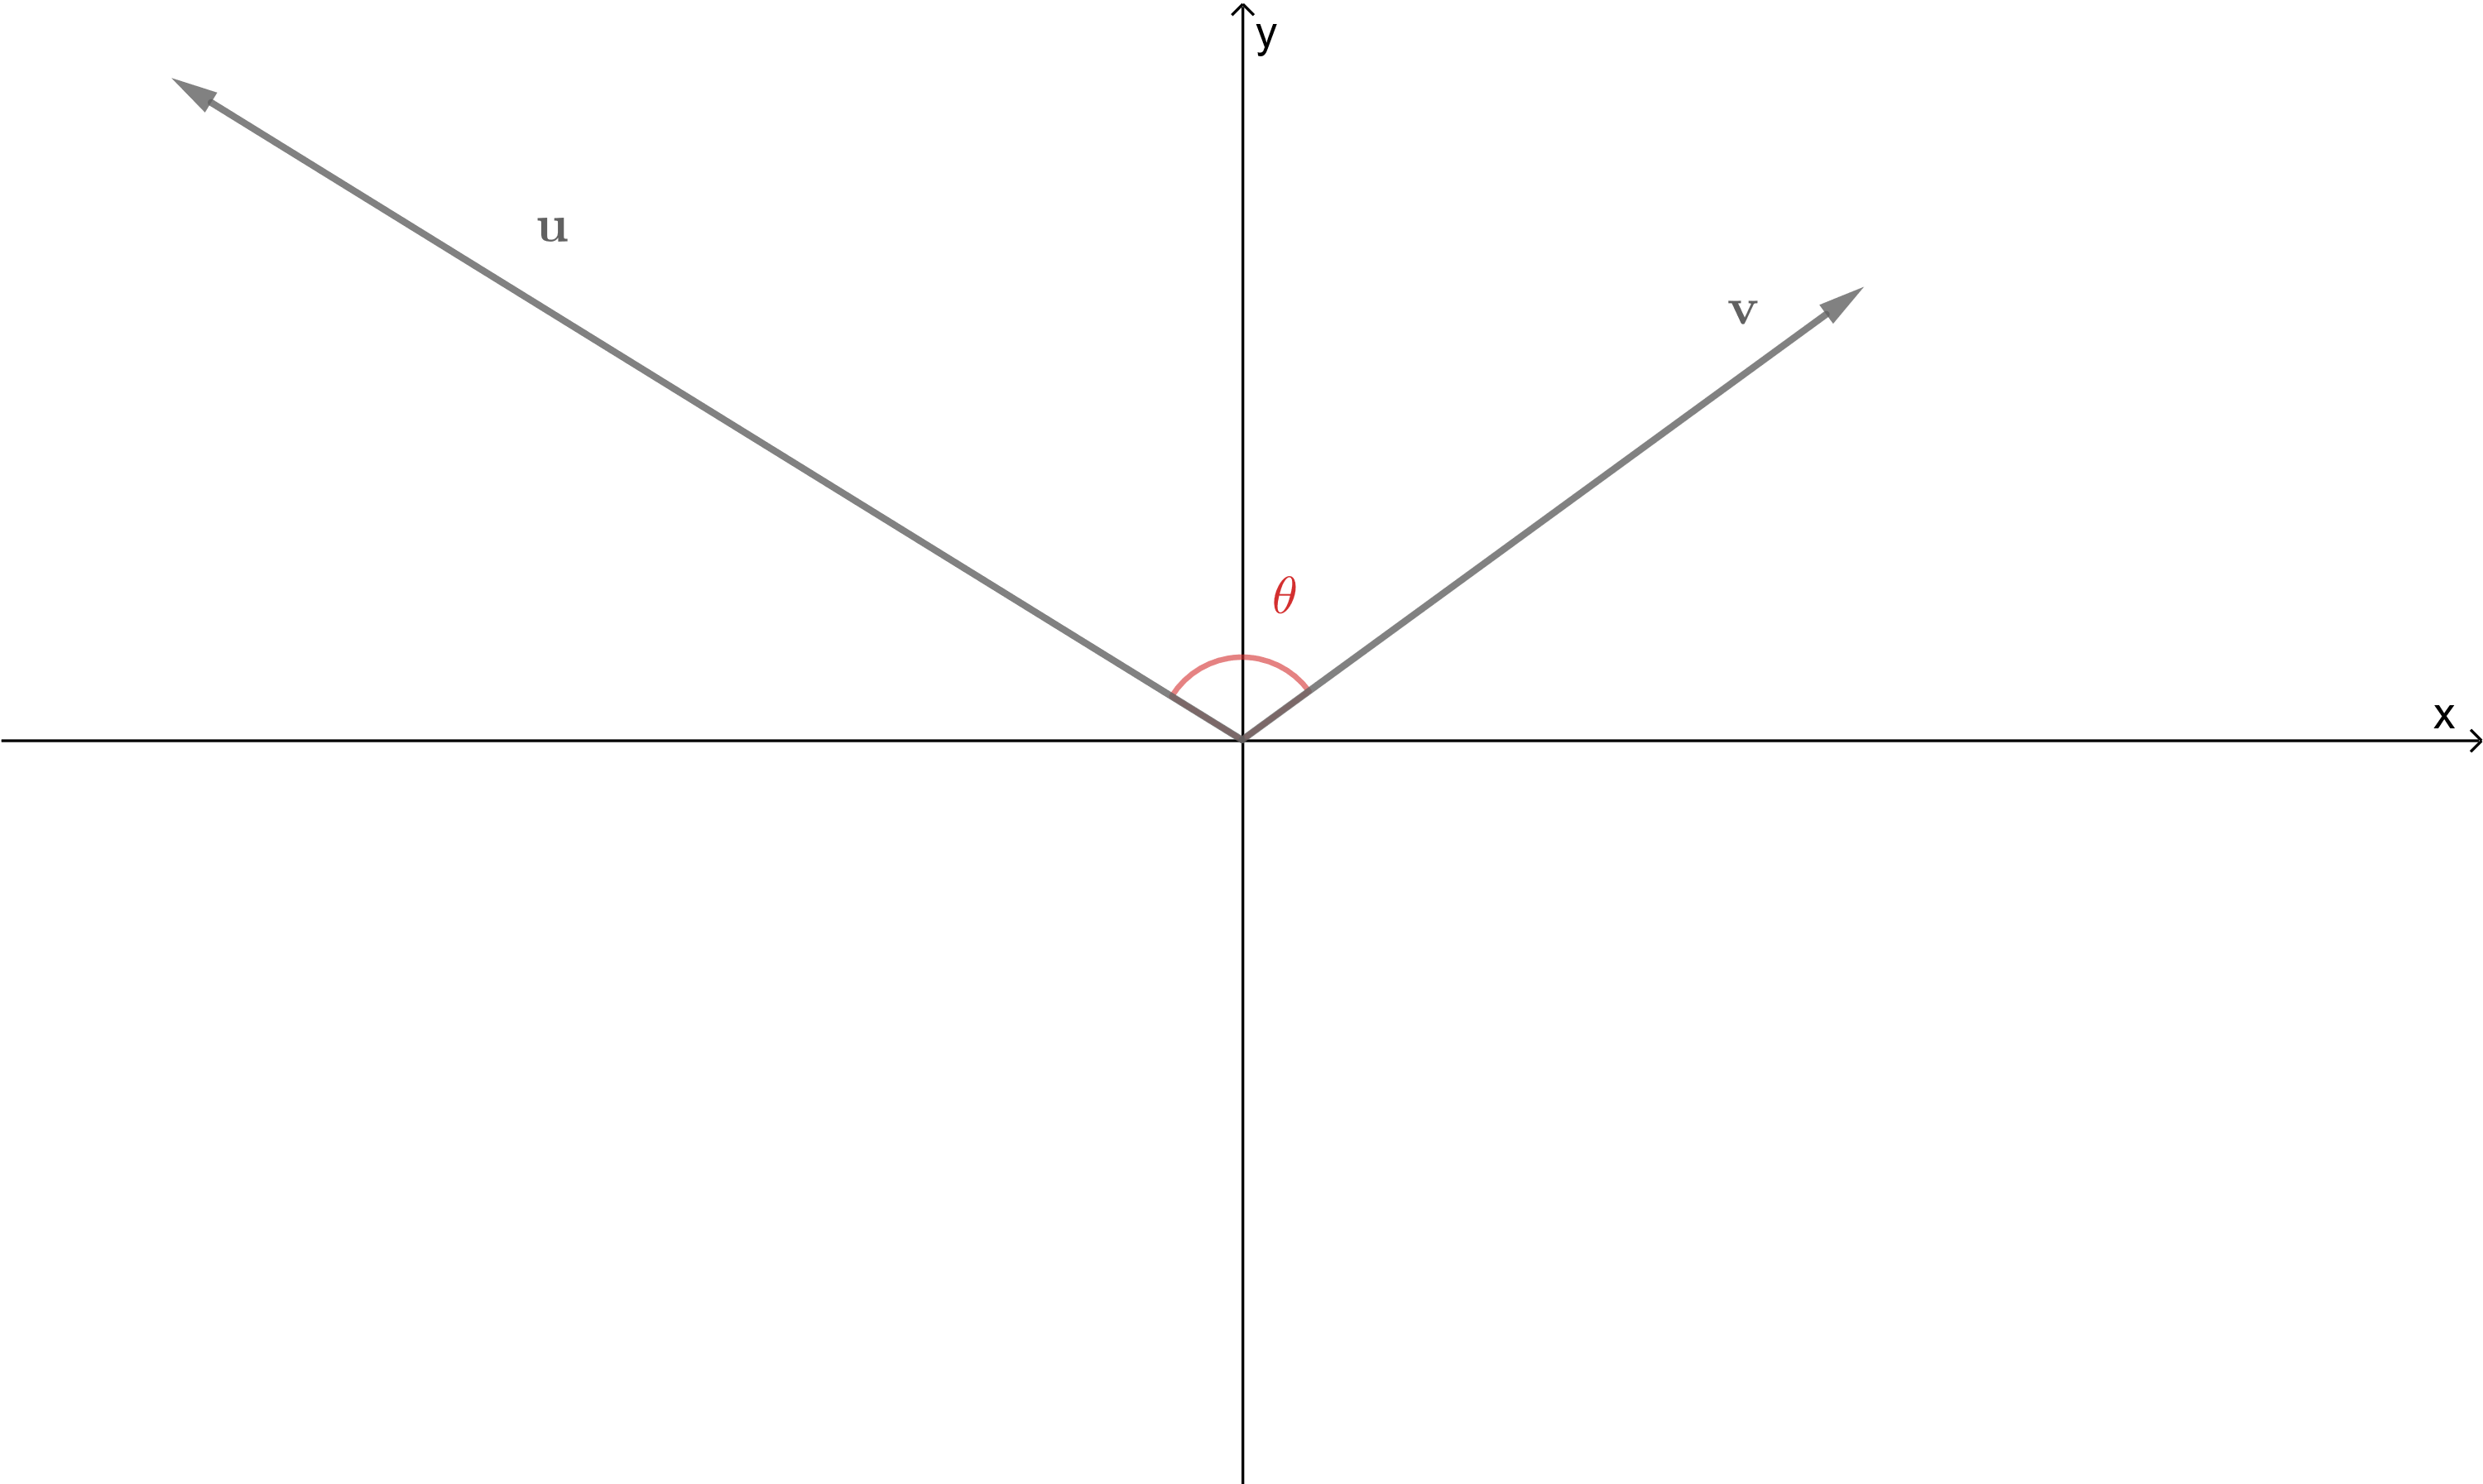
\includegraphics[width=0.7\textwidth]{anglebetween.png}
\end{figure}
How does $\mathbf u\cdot\mathbf v$ relate to this figure?
\pause
\[
\mathbf u\cdot\mathbf v = \norm{\mathbf u}\norm{\mathbf v}\cos\theta
\]
\end{frame}

\begin{frame}
\frametitle{Knowledge Checks}
\begin{figure}
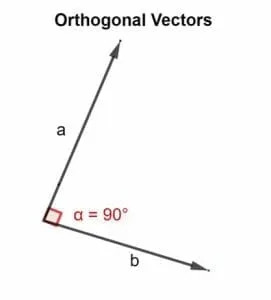
\includegraphics[width = 0.4\textwidth]{orthogonal-vectors.jpg}
\end{figure}
What is the dot product between a pair of orthogonal vectors? \pause
0
\end{frame}

\begin{frame}
\frametitle{Projections and vector components}
\begin{figure}
\centering
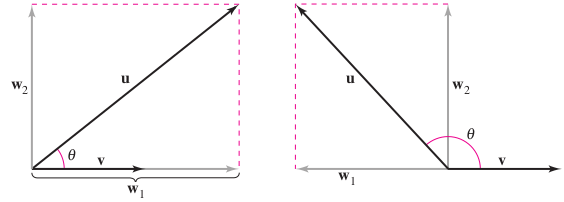
\includegraphics[width=1\textwidth]{projection2.png}
\end{figure}
What is $\mathbf w_1$ and $\mathbf w_2$ called?
\end{frame}

\begin{frame}
\frametitle{Projections and vector components}
\begin{figure}
\centering
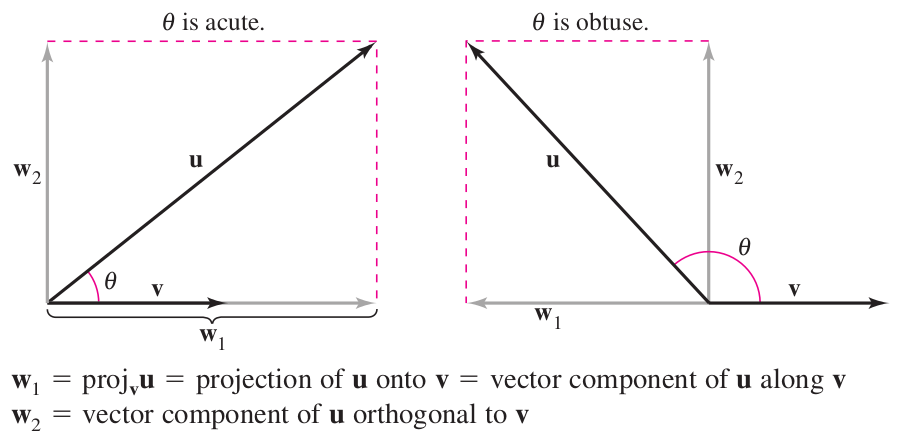
\includegraphics[width=1\textwidth]{projection.png}
\end{figure}
\pause
How to find $\mathbf w_1$ and $\mathbf w_2$?
\pause
\begin{align*}
\mathbf w_1 &= \left(\frac{\mathbf u\cdot\mathbf v}{\mathbf v\cdot\mathbf v}\right)\mathbf v\\
\mathbf w_2 &= \mathbf u - \mathbf w_1 = \mathbf u - \left(\frac{\mathbf u\cdot\mathbf v}{\mathbf v\cdot\mathbf v}\right)\mathbf v
\end{align*}
\end{frame}
\end{document}